\documentclass[12pt,titlepage]{article}

%% THE USEPACKAGES NECESSARY FOR THIS EXAMPLE
%% NOTE THAT genetics_manu_style MUST BE CALLED AFTER mychicago
\usepackage{graphicx}
\usepackage{endfloat}
\usepackage{amsfonts}
\usepackage{mychicago}
\usepackage{subfigure}
\usepackage{genetics_manu_style}
\usepackage{authblk} % improved citations
\usepackage{setspace} %double spacing
\usepackage{lineno} % line numbers
\usepackage{booktabs} % book-quality tables
\usepackage{multicol} % list corresponding authors in two separate columns
\usepackage{hyperref} % web links

%% Probably unnecessary packages.
\usepackage[T1]{fontenc}
\usepackage{lmodern}
\usepackage{amssymb,amsmath}
\usepackage{ifxetex,ifluatex}
\usepackage{fixltx2e} % provides \textsubscript




%% THE MANUSCRIPT TITLE
\title{Omics-based Single Step Trait Prediction}


% Allow for multiple authors to share the same institution.
\newcommand*\samethanks[1][\value{footnote}]{\footnotemark[#1]}

\author{
  Matthias Westhues\thanks{Institute of Plant Breeding, Seed Science and Population Genetics, University of Hohenheim, 70599 Stuttgart, Germany},
  Claas Heuer\thanks{Institute of Animal Breeding and Husbandry, Christian-Albrechts-University Kiel, 24098 Kiel, Germany},
  Georg Thaller\samethanks[2],
  Rohan Fernando\thanks{Department of Animal Science, Iowa State University, 50011 Ames, Iowa, U.S.A.},
  Albrecht E. Melchinger\samethanks[1]
}


\renewcommand{\CorrespondingAddress}{%
    University of Hohenheim \\
    Institute of Plant Breeding, Seed Science and Population Genetics \\ 
    Fruwirthstr. 21 \\ 
    Stuttgart 70599, GERMANY \\
    Tel.: (+49) 0711 459--22334 \\
    Fax: (+49) 0711 459--22343 \\ 
    \texttt{melchinger@uni-hohenheim.de} \vfill}

\renewcommand{\RunningHead}{Single Step Prediction}
\renewcommand{\CorrespondingAuthor}{Prof. Dr. A. E. Melchinger}
\renewcommand{\KeyWords}{single step, omics, prediction, maize}




%% SOME COMMANDS FOR THE CONTENT OF THIS FILE.  NOT NECESSARY FOR
%% GENETIC_MANU_STYLE
\newcommand{\bp}{\mathbf{p}}
\newcommand{\LLL}{\mathcal{L}}




%% BEGIN DOC
\begin{document}


\maketitle
\doublespacing
\linenumbers



\begin{abstract}

  $\dots$

\end{abstract}



% Please add here a significance statement to explain the relevance of your work
\section{Article Summary}
$\dots$



% Introduction
\section{Introduction}
% Rationale for predictions.
Genomic prediction, pioneered by \citeNP{Meuwissen2001}, has revolutionized
animal and plant breeding by a more efficient selection of promising candidates 
without phenotypes~\cite{DeLosCampos2013,Garcia-Ruiz2016} and recently emerged
as an important tool in human diagnostics~\cite{DeLosCampos2010,Vazquez2016}.
Its use is largely motivated by the high costs and oftentimes long duration of 
phenotyping, which can be reduced when covering all genotypes with a predictor 
while limiting phenotyping to a few genotypes with high precision
\cite{Kadam2016}.
The performance of all other genotypes is then forecast using model parameters
obtained from thorough resampling routines applied to the subset of individuals 
with full information~\cite{Hastie2009}.
In animal breeding, genomic selection has increased the annual selection gain 
by $\approx$ 50--100\% for yield traits and by 300--400\% for traits with low 
heritability~\cite{Garcia-Ruiz2016}.

% Incomplete predictors.
Breeding programs --- particularly in animal breeding --- are characterized by
the presence of one predictor type, which is available for all recorded
genotypes while other predictors are incomplete in that they cover only a 
subset of all genotypes~\cite{Fragomeni2015}.
Usually, the complete predictor is pedigree information while genomic data are
the most prevalent incomplete predictor.
To utilize all available phenotypic information for model training, methods were 
developed that allowed for a combined use of genomic and pedigree information 
\cite{Hayes2009a,VanRaden2009}.

% Two-step prediction.
Initially, a two-step procedure was the most intuitive choice for accomplishing
this goal~\cite{VanRaden2009}.
The first step consists of conventionally estimating breeding values based on
pedigree relationships and the phenotypes of relatives.
Individuals with accurate breeding values out of the first step (that is, a
high number of offspring), enter the second step in which conventional breeding
values are regressed onto SNP genotypes.
The estimated model coefficients can then be used to predict genomic breeding 
values for solely genotyped and potentially very young individuals.
However, as the breeding values from step one enter the genomic prediction
model as phenotypes, one has to be careful about the residual error
distribution of such a model.
For instance, the range of the prediction errors will no longer be identically
distributed, \textit{i.e.}, they should be weighted differently or estimated 
individually~\cite{Aguilar2010}.
One popular approach to account for this problem is deregressing the breeding
values and weighting the residuals according to the prediction error variances
\cite{Garrick2009}.

% Workings and advantages of the single step procedure.
Independently from each other,~\citeNP{Legarra2009} and
\citeNP{Christensen2010} developed a single step BLUP method that blends the 
numerator relationship matrix $\mathbf{A}$ with the genomic relationship matrix
$\mathbf{G}$ in a mutual matrix $\mathbf{H}$ to use all predictor information
simultaneously.
Issues with this H-BLUP approach were the compatability of $\mathbf{A}$ with
$\mathbf{G}$~\cite{Christensen2012} and their weighting, which is not
trait-independent~\cite{Vitezica2011,Ashraf2016}.
\citeNP{Fernando2014} derived the equivalent single step marker-effect-model to 
the single step breeding value model of \citeNP{Legarra2009} and 
\citeNP{Christensen2010}, which does not require weights for $\mathbf{A}$ and 
$\mathbf{G}$ and allows implicit modeling of the imputation error's structure.


% -   Mention scarcity of data on single step prediction in plant populations.
In animal breeding, single step prediction, particularly H-BLUP, has already 
become a routine procedure~\cite{Legarra2014} but, to the best of our knowledge, 
has only been considered in plants in a study on wheat~\cite{Ashraf2016} and
white spruce lines, respectively~\cite{Ratcliffe2017}.
Our objectives were threefold: (1) Examine whether the single step prediction
framework can be transfered to plant hybrids, (2) explore the utility of single 
step predition with a quantitative predictor and (3) evaluate the impact of the
proporition of genotypes not covered by the incomplete predictor on predictive
ability.










\section{Materials and Methods}
\Genetics2level{Exp1}
To address objectives 2 and 3, a maize inbred line data set, subsequently
referred to as \textit{Exp1}, was used~\cite{Yang2014}.
\textit{Exp1} originally comprised 513 maize lines representing the global maize
diversity  and was reduced to the set of tropical and subtropical lines
($n = 211$) given that it is the largest of the four pre-classified
subgroups~\cite{Yang2014}.
All inbred lines were evaluated in five Chinese environments ranging from
$18$ to $30^{\circ}$N and from $102$ to $110^{\circ}$E~\cite{Yang2014}.
Best linear unbiased predictors (BLUPs) were calculated for 17 traits of which 
six are presented in this study (Table~\ref{table:TraitKey}).
The selection of these traits was done so that four traits were better 
predicted by transcriptomic data and two further traits were better predicted 
by genomic data.
MaizeSNP50 BeadChip-data were available for the entire set of lines from the
diversity panel.
Additionally, RNA sequencing was performed for 368 lines on young seedlings 15 
days after sowing.
By exploiting identity by descent (IBD) between 49,728 SNPs on the BeadChip 
overlapping with the RNA-seq data, 556,809 high quality SNPs could be inferred 
for these lines~\cite{Fu2013,Li2013}.
For the remaining 145 maize lines without RNA-seq data, high density markers
were inferred via projection of IBD regions onto the BeadChip, using this core 
set of markers~\cite{Yang2014}.
The same SNP quality checks as for the parental inbred lines of the hybrids
were applied to the 211 inbred lines from the tropical/subtropical subset,
yielding 37,760 SNPs.
Gene expression data were normalized using a normal quantile transformation to
satisfy modeling assumptions~\cite{Fu2013}.
A subset of 28,850 annotated genes was available for 149 out of the 211
genotypes and was kept for further analyses~\cite{Li2013}.


\Genetics2level{Exp2}
To address objectives 1 and 2, a maize hybrid data set, subsequently
denoted as \textit{Exp2}, was used.
The material comprised 1,521 hybrids produced in 16 factorial mating designs
between 142 Dent and 103 Flint parent lines~\cite{Westhues2017}. 
Best linear unbiased estimates (BLUEs) were computed across all factorials and 
three or more agro-ecologically diverse locations across Germany for seven
agronomically important traits by accounting for year, location, field 
replication, block and genotype effects as well as their interactions
(Table~\ref{table:TraitKey}).
All 245 parent lines have pedigree records back to the generation of their 
grandparents or deeper~\cite{Westhues2017} and were genotyped using the Illumina 
BeadChip MaizeSNP50~\cite{Ganal2011}.
After filtering for minor allele frequency ($\geq 5$\%), heterozygosity rate
($\leq 5$\%) and call frequency ($\geq 95$\%), missing genotypes were imputed 
using the Beagle software~\cite{Browning2009}.
The final number of polymorphic marker loci was 7,013 for the Dent and 6,212 for 
the Flint lines, respectively.
Gene expression data for seedlings seven days after sowing were obtained for a 
subset of 60 Dent and 43 Flint lines, that are parents of 685 hybrid progeny.
These data were obtained through two-color hybridizations using a custom 2K 
microarray (GPL22267)~\cite{Westhues2017}.
After applying established normalization procedures~\cite{Smyth2003,Ritchie2007},
BLUEs for gene expression were computed for 1,323 transcripts while adjusting
for putative effects arising from the presence of multiple factorials
(\textit{cf.} \citeNP{Westhues2017}) using the R-package
\textit{limma}~\cite{Ritchie2015a}.




% Please add the following required packages to your document preamble:
% \usepackage{booktabs}
\begin{table}[]
\centering
\caption{Acronyms for the trait names}
\label{table:TraitKey}
\begin{tabular}{@{}lll@{}}
\toprule
Trait              & Abbreviation & Data Set  \\ \midrule
Cob weight         & CW           & Diversity \\
Days to silking    & DS           & Diversity \\
Ear diameter       & ED           & Diversity \\
100-grain weight   & GW           & Diversity \\
Kernel width       & KW           & Diversity \\
Plant height       & PH           & Diversity \\
Dry matter yield   & DMY          & Hybrid    \\
Dry matter content & DMC          & Hybrid    \\
Lignin             & ADL          & Hybrid    \\
Fat                & FAT          & Hybrid    \\
Protein            & PRO          & Hybrid    \\
Starch             & STA          & Hybrid    \\
Sugar              & SUG          & Hybrid    \\ \bottomrule
\end{tabular}
\end{table}


\Genetics2level{Population structure}
Population structure in \textit{Exp1} was examined by running a STRUCTURE
\cite{Pritchard2000} analysis with the number of putative ancestral
populations $K$ ranging from 2 to 9.
Based on the estimated probability of the data for each $K$, we chose $K=4$
and ran a principal component analysis (PCA) on the scaled and centered
genomic feature matrix using the \emph{pca} function from the \emph{R}-package
\emph{LEA} \cite{Frichot2015}.
Least-squares estimates of ancestry proportions were estimated based on sparse 
nonnegative matrix factorization algorithms~\cite{Frichot2014} using the 
\emph{snmf} function in \emph{LEA}.
Genotypes in the PCA plot (Fig.~\ref{fig:inbred-pca}) were colorized based on their
primary assignment to any of the four putative ancestral populations.
To avoid inflated predictive abilities, which can arise from large differences
in the average performance of the different subpopulations
\cite{Windhausen2012}, we reduced the panel of inbred lines to those primarily
belonging to either cluster 1 or cluster 4 in Fig.~\ref{fig:inbred-pca}.
This reduction yielded 164 genotypes, 110 of which were covered by both, genomic
and transcriptomic data.


\begin{figure}[H]
  \centering
  \includegraphics{./tables_figures/inbred_pca.pdf}
  \caption{
  Principal component analysis of 211 genotypes from the set
  `tropical/subtropical' of the maize diversity panel inbred lines.
  The four clusters are based on $K=4$ putative ancestral populations from a
  STRUCTURE analysis of the corresponding genomic feature matrix.
  Genotypes are colored based on their primary assignment to any of these four
  clusters.
}
\label{fig:inbred-pca}
\end{figure}



\Genetics2level{Prediction}
\subsection{Kernels}
BLUP models are computationally attractive when the number of features $p$
exceeds the number of genotypes $n$ and are equivalent to a selection index
when fixed effects have been accomodated by the dependent variable 
\cite{Mrode2014}.
Depending on the data set, up to three predictors were available for agronomic
trait predictions, namely pedigree data (P), genomic data (G) and
transcriptompic data (T).
The corresponding feature matrix of the $l$-th group of inbred lines 
($\mathbf{W}_{l}$) has dimensions $n_{l} \times p$ where $n_{l}$ pertains to 
the number of genotypes in the $l$-th group and $p$ pertains to the number of 
features.
Note that $l$ is only defined for \textit{Exp2} where a distinction between 
the two heterotic groups is necessary whereas $l$ can be ignored for all 
models pertaining to the inbred lines of the maize diversity panel in 
\textit{Exp1}.
For the diversity panel maize lines, $n_{l}$ corresponds to the number of 
genotypes whereas, in the case of the hybrid data, $n_{l}$ corresponds to the 
number of parent lines in the $l$-th heterotic group.
In generating kernels for each predictor, all features in $\mathbf{W}_{l}$ were
centered and standardized to unit variance.
Then, each kernel can be defined as

\begin{equation} \label{eq:GenomicRelationship}
  \mathbf{K}_{l} = \frac{1}{W_{l}} \mathbf{W}_{l} \mathbf{W}_{l}^{\top},
\end{equation}

where $W_{l}$ denotes the number of features~\cite{VanRaden2008}.
In the case of pedigree data (P), coancestry coefficients were used directly
for $\mathbf{K}_{l}$.


\subsection{Breeding value model}
The general model for breeding values was:

\begin{equation} \label{eq:KBLUPModel}
  \mathbf{y} = \mu + 
  \sum_{l=1}^{L} \mathbf{Z}_{l} \mathbf{g}_{l} + \mathbf{e},
\end{equation}

where $\mathbf{y}$ is the vector of observed inbred line or hybrid performance,
respectively, $\mu$ is the fixed model intercept, and $\mathbf{e}$ is the 
residual error.
For the hybrid data from \textit{Exp2}, we fit separate additive effects for 
each of the $L$ heterotic groups and $\mathbf{g}_{l}$ now pertains to the 
general combining ability effects of the parental inbred lines (either Dent or 
Flint, as expressed by $l$).
For the maize diversity panel inbred lines from \textit{Exp1}, we fit random 
genotype effects $\mathbf{g}_{l}$ (\textit{i.e.}, breeding values).
For both experiments, genetic effects $\mathbf{g}_{l}$ are associated with 
the vector of phenotypic performance $\mathbf{y}$ through a corresponding 
design matrix $\mathbf{Z}_{l}$.
The random effects ($\mathbf{g}_{l}$) have expectation zero and variance equal 
to $\mathbf{K}_{l} \sigma^{2}_{{g}^{l}}$ and $\mathbf{I} \sigma^2_{e}$ 
for the residual error.
Here, we did not consider the inclusion of dominance effects for the hybrid
material after a previous investigation into the predictive ability of various
``omics'' predictors in the same material concluded no considerably gains 
\cite{Westhues2017}.
All prediction models were implemented using the R-packages \textit{BGLR}
\cite{Perez2014} and \textit{sspredr}
\url{https://github.com/mwesthues/sspredr}.


\subsection{Single step prediction}
For simplicity, let us assume throughout this section that we have $L=1$.
If the breeding values are fully captured by the features in $\mathbf{W}$,
Eq.~\ref{eq:KBLUPModel} can then be expressed as

\begin{align} \label{eq:KBLUPModelSimplified}
	\mathbf{y} &= \mu + \mathbf{Z} \mathbf{g} + \boldsymbol{e} \\
	&= \mu + \mathbf{Z} \mathbf{W} \boldsymbol{\alpha} + \boldsymbol{e}
\end{align}
\cite{Fernando2014} since the ridge regression model is equivalent to the BLUP
model~\cite{Ruppert2003}.


Hence, the breeding values in a prediction model are given by:
\begin{equation} \label{eq:mrnaebv}
	\mathbf{\hat{g}} = \mathbf{W}\boldsymbol{\hat{\alpha}},
\end{equation}

where $\boldsymbol{\hat{\alpha}}$ is the solution to a ridge regression model.

Consider now the situation in which one predictor is complete in the sense that
the whole population is equipped with features for that predictor whereas only
a subset of that population has information on a second predictor.
We can take a similar route as in \citeNP{Fernando2014} and impute covariates 
of the incomplete predictor by using covariates of the complete predictor.
Let the subscript $1$ denote individuals covered only by the complete
predictor whereas individuals covered by both, the complete and the
incomplete predictor, are indicated by the subscript $2$.
Further, the covariates in $\mathbf{W}$ are centered.
In this case we need to partition the vector of breeding values $\mathbf{g}$
into a component $\mathbf{g}_{1}$ (\textit{i.e.,} breeding values of animals 
covered only by the complete predictor) and a component 
$\mathbf{g}_{2} = \mathbf{W}_{2}\boldsymbol{\alpha}$ (\textit{i.e.,} breeding 
values of animals covered by both predictors).
Under multivariate normality, the vector $\mathbf{g}_1$ can be written as the
sum of the conditional expectation given $\mathbf{g}_2$ and a residual error
term:
\begin{align} \label{eq:mrna1}
	\mathbf{g_1} &= E(\mathbf{g}_1|\mathbf{g}_2) + \boldsymbol{\epsilon} \\
	&= \mathbf{K_{12}}\mathbf{K_{22}}^{-1}\mathbf{W_2}\boldsymbol{\hat{\alpha}} + (\mathbf{g_1} - \mathbf{K_{12}}\mathbf{K_{22}}^{-1}\mathbf{W_2}\boldsymbol{\hat{\alpha}}) \\
	&= \mathbf{\hat{g}}_1 + \boldsymbol{\epsilon},
\end{align}

where $\mathbf{K}_{ij}$ are partitions of $\mathbf{K}$ that correspond to 
$\mathbf{g}_{1}$ and $\mathbf{g}_{2}$, respectively~\cite{Fernando2014}.

The covariance matrix of $\boldsymbol{\epsilon}$ is $\mathbf{K}_{11} - \mathbf{K}_{12}\mathbf{K}_{22}^{-1}\mathbf{K}_{21} = (\mathbf{K}^{11})^{-1}$
\cite{Legarra2009}.

The structure of the residual imputation/prediction error is known and can 
therefore be modeled.

The general model for the single step procedure can then be written as 

\begin{equation} \label{eq:single-step-model}
\mathbf{y} = \mathbf{Xb} + \mathbf{W} \boldsymbol{\alpha} + \mathbf{U} \boldsymbol{\epsilon} + \mathbf{e},
\end{equation}

with

\begin{equation} \label{eq:single-step-submatrices}
\mathbf{X} = 
\begin{bmatrix}
  X_1 \\
  X_2 
 \end{bmatrix},
 \mathbf{W} = 
\begin{bmatrix}
  Z_1\hat{\mathbf{W}_1} \\
  \mathbf{W}_2 
 \end{bmatrix},
 \mathbf{U} = 
\begin{bmatrix}
  Z_1 \\
  0 
 \end{bmatrix},
\end{equation}

where $\hat{\mathbf{W}}_{1} = \mathbf{K}_{12} \mathbf{K}_{22}^{-1} \mathbf{W}_{2}$.

Following the notation in \citeNP{Fernando2014} the phenotypes can be untangled 
as:

\begin{align} \label{eq:entangled-augmented-single-step-model}
\begin{bmatrix}
  y_1 \\
  y_2 
 \end{bmatrix}
& =
 \begin{bmatrix}
  X_1 \\
  X_2 
 \end{bmatrix}
 \boldsymbol{\beta} + 
 \begin{bmatrix}
  Z_1 & 0 \\
  0 & Z_2 
 \end{bmatrix}
\begin{bmatrix}
  g_1 \\
  g_2 
 \end{bmatrix}
  + \mathbf{e} \\
    & = 
 \begin{bmatrix}
  X_1 \\
  X_2 
 \end{bmatrix}
 \boldsymbol{\beta} + 
 \begin{bmatrix}
  Z_1 & 0 \\
  0 & Z_2 
 \end{bmatrix}
\begin{bmatrix}
  \mathbf{K}_{12}\mathbf{K}_{22}^{-1}\mathbf{W}_2\boldsymbol{\alpha} + \boldsymbol{\epsilon}  \\
  \mathbf{W}_2\boldsymbol{\alpha} \\
 \end{bmatrix}
  + \mathbf{e} \\
    & = 
 \begin{bmatrix}
  X_1 \\
  X_2 
 \end{bmatrix}
 \boldsymbol{\beta} + 
 \begin{bmatrix}
  Z_1 & 0 \\
  0 & Z_2 
 \end{bmatrix}
\begin{bmatrix}
  \hat{\mathbf{W}_1}\boldsymbol{\alpha} + \boldsymbol{\epsilon} \\
  \mathbf{W}_2\boldsymbol{\alpha} \\
 \end{bmatrix}
  + \mathbf{e} \\
\end{align}


Our final model looks like this:

\begin{align} \label{eq:final-model}
\mathbf{y} &= \mathbf{Xb} +
\sum_{l=1}^{L} \mathbf{Z}_{l}\mathbf{W}_{l} \boldsymbol{\alpha}_{l} + 
\sum_{l=1}^{L} \mathbf{Z}_{l}\mathbf{U}_{l} \boldsymbol{\epsilon}_{l} +
\mathbf{e}.
\end{align}


Breeding values or general combining abilities can be estimated as:

\begin{equation} \label{eq:breeding-values}
\hat{\mathbf{g}} = 
 \begin{bmatrix}
  \hat{\mathbf{W}_1} \\
  \mathbf{W}_2 
 \end{bmatrix}
 \hat{\boldsymbol{\alpha}}
 + 
 \begin{bmatrix}
  \mathbf{Z}_1 \\
  0
 \end{bmatrix}
 \hat{\boldsymbol{\epsilon}} 
\end{equation}

For the hybrid data, the obtained GCA effects for the inbred lines represent 
half their breeding values.
The predicted agronomic performance is:

\begin{equation} \label{eq:predicted-performance}
\hat{\mathbf{y}} = \sum_{l=1}^{L} \mathbf{Z}_{l}\hat{\mathbf{g}}_{l} 
\end{equation}


\subsection{Predictive ability and model validation}
For the validation of our predictions, we employed leave-one-out
cross-validation (LOOCV) routines.
In the case of the diversity panel maize inbred lines, LOOCV was performed by 
using a single genotype as a hold-out sample, which will be predicted by using
all other inbred lines for model training.
This process is repeated until all inbred lines have been used once for testing
and $n - 1$ times for model training.

For the hybrid data, LOOCV was carried out as follows:
Let $D$ and $F$ denote the set of parental inbred lines from the Dent and the 
Flint group, respectively.
Further, let $H \cap [D \times F]$ denote the set of hybrids from crosses 
between $D$ and $F$.
Let $H_{i \times j}$ denote the test set hybrid to be predicted.
We can then define the parents of the training set hybrids as
$D_{i} = D \setminus \{i\}$ and $F_{j} = F \setminus \{j\}$, respectively.
The training set is then defined as 
$H_{TRN}(x \times j) = H \cap (D_{i} \times F_{j})$.

We judged the performance of each model by looking at its predictive ability,
which is calculated as $\rho(\mathbf{y}, \mathbf{\hat{y}})$, where 
$\mathbf{\hat{y}}$ is the vector of predicted values from each LOOCV run.

Standard errors for the predictive abilities were calculated by bootstrapping
predictive and observed values 1,000 times using the \emph{R} package 
\emph{boot}~\cite{Canty2017}.



\Genetics2level{Core sampling}
In order to evaluate the influence of the fraction of genotypes that is not
covered by the incomplete predictor on predictive ability we generated core
sets of nine different sizes from \textit{Exp1}
(Fig.~\ref{fig:compound-plot}~a).
The base of each of these core sets was the superset of genotypes that were
covered by both, genomic and trancriptomic data.
A core set was created by artificially declaring a pre-specified fraction 
$x = {10\%, 20\%, \dots, 90\%}$ of genotypes as lacking of transcriptomic 
information.
For each value of $x$ we created 100 core sets $s \in {1, 2, 3, \dots, 100}$ by
repeatedly sampling genotypes, whose trancsriptomic information was declared
as missing, at random (Fig.~\ref{fig:compound-plot}~b).
The artificially removed transriptomic information on these genotypes was then
imputed.

\begin{figure}[H]
  \centering
  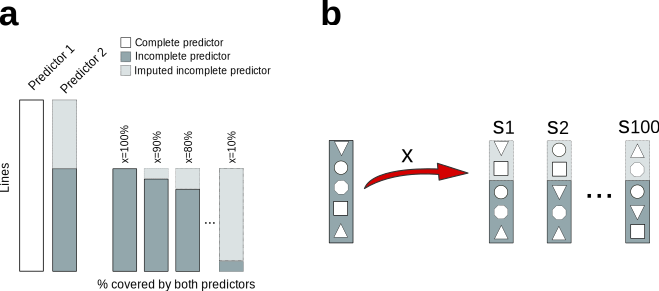
\includegraphics[width=1\textwidth]{./tables_figures/compound_plot.pdf}
  \caption{
  (\textbf{a}) Scheme for the amount of genotypes covered by predictors.
  The two extended bars represent the entire set of genotypes in either
  \textit{Exp2} or \textit{Exp1}.
  All genotypes are covered by at least one predictor, which is called the
  `complete' predictor and depicted as a white bar.
  The second bar shows that only a fraction of genotypes is covered by both,
  the `complete' and the `incomplete' predictor (dark gray) and that the
  difference between the predictors will be imputed (light gray fraction).
  The four bars to the right outline the principle of generating core sets for
  \textit{Exp1}.
  For nine different values of $x$, which represents the fraction of genotypes
  covered by the `incomplete' predictor, core sets are build.
  (\textbf{b}) Subsampling within core sets.
  Each of the black symbols represents a different genotype.
  For each value of $x$, 100 subsets $s$ are generated where $x\%$ of genotypes
  are randomly declared to be covered by both, the `complete' and the
  `incomplete' predictor whereas the remaining $100\% - x\%$ of genotypes
  are declared to be covered only by the `complete' predictor.
  }
\label{fig:compound-plot}
\end{figure}



\section*{Results}
\Genetics2level{Exp1}
At the level of the 110 genotypes for which both, genomic (G) and 
transcriptomic (T) information, were available, the use of T yielded higher
predictive abilities than the use of G for two out of six traits
(Fig.~\ref{fig:InbredResults}A).
In terms of predictive ability, the absolute advantage of T over G was as large 
as 0.15 as observed for the trait ED\@.
The predictive ability for predictions based on G were always higher for the
full set of inbred lines ($n = 164$) than for the reduced set of inbred lines
($n = 110$).
The combination of G and T (\textit{i.e.}, GT) in a single-step approach for the 
prediction of all 164 lines, performed at least as well as G alone when T was 
superior over G for the reduced set of 110 lines.
In the case of KW and ED, the use of GT yielded a slight improvement in predictive 
ability over G.
Where T was a worse predictor for the reduced set of 110 lines than G,
predictive abilities of GT for the full set of 164 lines were also worse than 
those based on G alone.

\begin{figure}[H]
  \centering
  \includegraphics{./tables_figures/pred_ability_inbred.pdf}
  \caption{
  Predictive abilities and average, bootstrapped standard errors for
  tropical/subtropical inbred lines from the maize diversity panel and six
  agronomic traits.
  As predictors, genomic (G) data, transcriptomic (T) data and their 
  combination (GT) were used.
  The `Reduced' panel includes a subset of 110 lines covered by genomic and
  transcriptomic information whereas the `Full' panel comprises all 164
  genotypes.
  In the `Full' set of genotypes, transcriptomic records were imputed for 54
  lines.
  }
\label{fig:InbredResults}
\end{figure}



\Genetics2level{Exp2}
The maize hybrid data set contains information on seven agronomic traits and
three predictors, namely pedigree data (P), genomic information (G), 
transcriptomic information (T), and combinations thereof.
Pedigree records and genomic information were available for the 245 parent 
lines of all 1,521 hybrids and we denote these data as the `Full' set whereas
transcriptomic data were available for 103 parent lines of 685 hybrids, which
we denote as `Reduced'.
In the `Reduced' set, transcriptomic data were the best single predictor for
ADL, PRO and particulaly for DMY where the predictive ability obtained with T
was 0.08 points higher than for G as the second best predictor for this trait
(Fig.~\ref{fig:HybridResults}).
In the reduced set, P had the highest predictive ability for STA and DMC\@.
For FAT and SUG, G was the superior predictor inside the reduced set.
In the full set of 1,521 hybrids, predictive abilities obtained with G rose 
markedly for all traits with the exception of FAT\@.
The combination of genomic and transriptomic information (GT) in a single-step
model yielded a small improvement over G alone for the traits DMY and PRO\@.
Except for PRO, compared to using only G, trait prediction did not benefit from 
the single step approach when T was not superior to G in the reduced set.
Predictive abilities resulting from combinations of pedigree with genomic (PG)
information were better than P alone for all traits and PT improved upon P in
the `full' set for four traits.

\begin{figure}[H]
\centering
  \includegraphics{./tables_figures/pred_ability_hybrid.pdf}
  \caption{
    Predictive abilities and average, bootstrapped standard errors for the set
    of maize hybrids and seven agronomic traits.
    As predictors, pedigree (P), genomic (G), transcriptomic (T) data and 
    combinations thereof we used.
    The `Full' set of genotypes comprises 1,521 hybrid progeny based on 245
    parental inbred lines, whereas the `Reduced' set comprises 685 hybrid
    progeny based on 103 parental inbred lines.
  }
\label{fig:HybridResults}
\end{figure}





\Genetics2level{Impact of coverage by the incomplete predictor}
Single-step approaches are based on the use of one complete predictor that
covers all genotypes and one incomplete predictor that covers only a subset of
all available genotypes.
Here, we explore the impact of which data are covered by the incomplete 
predictor on the predictive abilities obtained via single-step approaches by
focusing exclusively on the 110 inbred lines from the maize diversity panel
that are covered by both, genomic and transcriptomic information.
First, we assembled nine different core sets, each with 100 nested subsamples,
which were generated by randomly removing transcriptomic information from
some genotypes (Fig.~\ref{fig:compound-plot}).
The nine core sets differ in that each covers a different number of genotypes,
ranging from only 10\% to 90\% of all genotypes covered by the incomplete
predictor (Fig.~\ref{fig:inbred-pca}).

\begin{figure}[H]
  \centering
  \includegraphics{./tables_figures/pred_ability_inbred_core_fraction.pdf}
  \caption{
  Influence of the fraction of genotypes covered by the incomplete predictor
  on predictive abilities.
  Predictive abilities are based on transcriptomic effects derived from a
  single step prediction model involving transcriptomic (T) and genomic (G)
  data, respectively.
  Results are shown for the core set of 110 inbred lines from \textit{Exp1} for
  which both, G and T are available for any genotype and six agronomic traits.
  The fraction of genotypes (\textit{i.e.} `Core Fraction') for which
  T was available is given on the x-axis.
  Dotted lines indicate that $T > G$, dashed lines indicate that $T \approx G$
  and solid lines indicate that $G > T$ when running predictions using single
  predictors on the same data set.
  }
\label{fig:InbredResults}
\end{figure}


Predictive abilities obtained with the different core sets varied widely within
most traits (Fig.~\ref{fig:InbredResults}).
For most traits, an initial increase in predictive abilities when moving
from a core set size of 10\% to 20\%/30\% was observed, regardless of whether G
or T individually was the superior predictor.
For the traits CW, GW and PH, which were better predicted via G than via T in
the reduced set of lines, predictive abilities were higher when only a small
number of genotypes was included in the core set.
This corresponds to a situation where a large number of genotypes is being 
imputed and the majority of the information is derived from genomic information.
A hike in predictive abilities, when moving from a core fraction of 10\% to 
90\%, was observed for ED and KW, which were predicted better when using T
individually compared to using G individually.
The only trait that was barely affected by a change in the core fraction was DS
for which the predictive abilities using either G or T individually were almost
identical (Fig.~\ref{fig:InbredResults}).




\section*{Discussion}
\Genetics2level{Advantages of marker effect models}
Single step approaches in hybrid populations have so far been limited to pig
breeding~\cite{Xiang2015,Xiang2016,Tusell2016}.
All of these studies used breeding value-based single step BLUP methods
(SS-BLUP) conceived by \citeNP{Legarra2009} and \citeNP{Christensen2010} with
extensions to hybrid populations~\cite{Christensen2014,Christensen2015}.
An attactive property of SS-BLUP models is their computational advantage over 
marker-effect single step Bayesian regression models (SSBR) when the number of 
genotypes is smaller than the number of features of the incomplete predictor.
Nevertheless, SS-BLUP suffers from a variety of issues, which we will present
briefly:
First, the combination of the numerator with the genomic relationship matrix
requires commensurability of the two matrices, which necessitates some form of
scaling and weighting of $\mathbf{A}$ and $\mathbf{G}$
\cite{Christensen2012,Christensen2012a}.
Second, the fact that mostly recent individuals have genotypes whereas the 
majority of old individuals has only pedigree records introduces a bias that 
has to be accounted for~\cite{Vitezica2011,Legarra2015,Garcia-Baccino2017}.
Third, the addition of new genotypes requires updates of $\mathbf{G}$ that
demand additional measures such as computing the inverse of $\mathbf{G}$ via
recursion
\cite{Misztal2014,Misztal2016,Misztal2016a,Fragomeni2015,Masuda2016,Pocrnic2016}.
Advantages of the SSBR algorithm, conceived by \citeNP{Fernando2014}, include
that i) it does not require commensurability of $\mathbf{A}$ and $\mathbf{G}$, 
ii) it models the bias incurred by the incomplete predictor explicitly as 
$\mathbf{\epsilon}$ and iii) its speed depends largely on the number of 
features.
To our best knowledge, this study presents the first implementation of the SSBR 
algorithm on a hybrid data set.




\Genetics2level{Addition of new predictors}
Pedigree records are the most ubiquitous predictor in animal and plant breeding
programs, because they are easy and inexpensive to collect.
Compared to pedigree information, which represent the expected relationship
among individuals, genomic information capture Mendelian sampling and thereby 
provide an improved proxy of the realized relationship among individuals.
Nevertheless, genomic data do not exhaustively capture physiological epistasis 
\cite{Jiang2015,Guo2016,Vazquez2016}, describing the interactions 
within and between different biological strata~\cite{Sackton2016}.
Such interactions were found to be pervasive throughout the genomes of yeast 
\cite{Brem2005} and humans~\cite{Brown2014} and have motivated studies on the 
utility of downstream `omics' predictors for integrating such interactions.
Recently, encouraging results have been found for humans~\cite{Vazquez2016}, 
maize inbred lines~\cite{Guo2016} and maize hybrids~\cite{Westhues2017}.
While single step prediction has become an established method when complete
pedigree but only incomplete genomic records are available, its application has
not yet been considered for the imputation of a complete predictor based on 
incomplete downstream `omics' predictors such as transcriptomic, proteomic or 
metabolomic data.
Here, we considered single step approaches for a maize inbred line diversity
panel as well as for a collection of maize hybrids using pedigree, genomic and
transcriptomic data as predictors.


\Genetics2level{Superiority of single step models}
\subsection{Exp1}
When using a single step approach based on complete genomic and incomplete
transcriptomic information, gains in predictive ability for the inbred lines
were at best just slightly higher than when using complete genomic information
alone.
One of the reasons might be that the subset of genotypes that was covered by
transcriptomic data was not a good representation of the full genetic space of
all available genotypes.
Another possibility is that the number of additional phenotypes in the full
set compared to the reduced set ($\Delta(n) = 54$) was not large enough to
provide considerably more useful information.
The latter was the case for \citeNP{Ashraf2016}, who imputed genotypes for about 
10,000 wheat lines using pedigree information and observed greater accuracy of
the single step method over genomic BLUP for all four evaluated traits.
Predictive abilities reported for the maize diversity panel in this study were
slightly different from those reported by \citeNP{Guo2016}, for three
possible reasons:
1) We reduced the dataset to 164 tropical/subtropical lines with little evident
population structure and excluded all other genotypes from our analyses whereas
\citeNP{Guo2016} used genotypes from four different subpopulations, modeled as a
fixed effect.
2) We applied quality checks for the predictor data after generating the subset
of 164 inbred lines, whereas \citeNP{Guo2016} applied the quality checks to 368
genotypes.
3) While \citeNP{Guo2016} used five-fold cross-validation with 500 repetitions,
we employed a leave-one-out cross-validation scheme (LOOCV).
Notwithstanding, the relative differences between predictive abilities for G 
and T, respectively, were similar in both studies.


\subsection{Exp2}
Hybrid breeding --- with noteworthy commercial applications in pig
\cite{Xiang2016,Tusell2016} and maize breeding~\cite{TheRoyalSociety2009} --- 
is a particularly challenging application field for prediction tools 
\cite{Kadam2016}.
Here, $2n$ parent individuals from two genetically distinct heterotic groups are
crossed to each other, yielding $n^{2}$ potential hybrid progeny that would
require intensive field testing.
In medium-sized plant breeding programs, the advent of the doubled haploid (DH) 
technology~\cite{Wedzony2009} now allows for an annual production of 1,000 
parent lines in each heterotic group, amounting to $10^{6}$ putative hybrid
progeny.
\citeNP{Westhues2017} have shown that, in hybrid breeding, the probability 
of successfully selecting the best observed genotypes based on the best 
predicted candidates is a strongly convex function of the predictive ability.
Thus, even minor gains, when using transcriptomic and genomic data in a
single step, might justify additional investments in RNA-seq at least for a
subset of genotypes that represents the genetic space of the breeding 
material well.
For the hybrid data, the predictive abilities of genomic information
for the whole set of available parent lines rose considerably for several
agronomic traits.
Hence, the inclusion of trancsriptomic data could not further improve upon
genomic information alone.
Predictive abilities obtained when using pedigree data could be 
improved considerably when, depending on the agronomic trait, combined with 
either transcriptomic or genomic information.
This suggests that single step prediction should always be considered when the
incomplete predictor offers an appreciably higher predictive ability compared
to the complete predictor.


\Genetics2level{Coverage of the genetic space}
Whereas animal breeding populations are oftentimes so large that the assembly 
of a core set of individuals with records on multiple predictors can effectively 
be done at random once more than 10,000 animals have pedigree records 
\cite{Fragomeni2015,Lourenco2015,Masuda2016}, pedigrees in plant breeding 
programs are typically considerably smaller.
Single step prediction offers the promise of leveraging the predictive ability
for all genotypes by borrowing the superior performance of an auxiliary
predictor on only a subset of genotypes, thereby reducing predictor costs.
Hence, we were interested in determining to what extent individuals should be 
complemented with information on another predictor.
By randomly and repeatedly declaring trancsriptomic information missing from
genotypes in \textit{Exp1} we examined how reliably single step prediction works
depending on the fraction of genotypes covered by both, the complete and the
incomplete predictor.
We observed that about $20-30\%$ of genotypes needed to be covered by both
predictors to match the performance achieved with the complete predictor
individually.
Beyond this fraction of covered genotypes the trend in predictive ability
changes was stable.



\section*{Conclusions}
We successfully applied single step prediction to a hybrid plant data set 
while imputing with a quantitative downstream `omics' predictor.
By declaring different subsets of individuals as covered by one or two 
predictors, respectively, we could elucidate the influence of differences
between two predictors on predictive ability when used in a single step
approach.
When the discrepancy in predictive ability between the complete and the
incomplete predictor was skewed profoundly in favor of the incomplete predictor,
such as for pedigree and transcriptomic data, single step prediction was shown
to be highly beneficial.
Extensions to more than two predictors were outside the scope of this study
but, with mounting interest in systems genetics, should be considered in the
future.





\section{Acknowledgments}
This project was funded by the German Federal Ministry of Education and 
Research (BMBF) within the projects OPTIMAL (FKZ: 0315958B,0315958F),
SYNBREED (FKZ: 0315528D) and by the German Research Foundation 
(DFG, Grants No. ME 2260/5-1 and SCHO 764/6-1).
The authors acknowledge support by the state of Baden-W{\"u}rttemberg through 
bwHPC\@.
Financial support for M.W. was provided by the Fiat Panis foundation, Ulm,
Germany.



\nolinenumbers
% Bibliography
\bibliography{library}
\bibliographystyle{mychicago}
\end{document}
